\section{Diseño y arquitectura}

Se detalla a continuación las decisiones que se tomaron para solucionar los aspectos más importantes de diseño
y la arquitectura de comunicación con el resto de las aplicaciones.

Como criterio general, se intentó siempre permitir el mayor grado de independencia posible entre el administrador
y cada aplicación. Esto significa no sólo que cada aplicación pudiera escoger su propia forma de almacenar los
datos, sino que también se pudiera implementar la comunicación con el administrador de identidades en una aplicación
cualquiera de forma sencilla, sin imponer restricciones excesivas sobre nuevas tecnologías a integrar.

\subsection{Almacenamiento de claves}

Posiblemente el principal problema a resolver fue el de cómo se iban a almacenar las claves. La primera restricción
surgía del requerimiento de que cada aplicación debía poder utilizar un mecanismo de autenticación propio.

Inicalmente, la solución más sencilla parecía ser que, al registrarse un usuario o cambiar su clave, se enviara
la misma a través de un canal seguro en texto plano. Al recibir una nueva clave, cada aplicación cliente podría
almacenarla en el formato que prefiera. De esta forma, el administrador sólo debería guardar la clave de una forma
(la que se eligiera utilizar para la autenticación al mismo administrador).

Siempre y cuando se pudiese confiar en el canal de transmisión, esta alternativa parecía bastane acertada:
brindaba independencia total entre el administrador y la forma de almacenar las claves de cada aplicación.
Sin embargo, se tiene el problema de que al agregar una nueva aplicación al administrador no habría forma de
informarle las credenciales de los usuarios previamente existentes. Dado que en esta situación no es viable
forzar a todos los usuarios a cambiar sus claves, se descartó esta posibilidad.

Una modificación ingenua sobre lo anterior hubiese sido seguir enviando las claves a las otras aplicaciones 
en texto plano, pero esta vez guardándolas también en el administrador utilizando algún tipo de cifrado reversible.
De esta forma, se podría obtener las claves de los usuarios en cualquier momento con el fin de enviarlos a
otras aplicaciones. Aparte de las consideraciones adicionales de implementación que representaría, la principal
desventaja de esta opción es que en caso de comprometerse la clave de cifrado se estarían conociendo inmediatamente
las claves de todos los usuarios.

Finalmente se terminó optando por almacenar utilizando varios mecanismos de hash distintos. En primer lugar,
esto requiere definir previamente cuáles son los algortimos soportados. También necesariamente el administrador
de identidades debera conocer qué mecanismo de almacenamiento de claves utiliza cada aplicación. Si bien esto
es una pérdia de independencia con respecto a la implementación de las aplicaciones, soluciona el problema 
anterior: siempre se cuenta con la clave en el \textit{formato}.

Observamos de todos modos dos desventajas en la alternativa elegida:
\begin{itemize}
 \item  En cierto modo, nuestra forma de almacenar las claves será tan débil como el mínimo que se ofrezca al
 		resto de las aplicaciones. De todos modos, si bien es cierto que se impone un techo sobre la seguridad
 		del mecanismo de almacenamiento, consideramos razonable asumir que el sistema se implementaría en
 		organizaciones donde se determina un nivel de seguridad mínimo para el tratamiento de datos sensibles,
 		por lo cuál este techo del que hablábamos antes no debería ser muy bajo: no se deberían ofrecer opciones
 		que se consideren inseguras.
 \item  La opción inicial tenía la ventaja de que el administrador no necesitaba conocer cómo las aplicaciones
 		almacenaban sus claves. Esto permitía que no hiciera falta hacer ningún cambio en caso de de agregarse
 		una aplicación con un mecanismo de almacenamiento no conocido hasta el momento. Con la alternativa
 		elegida, no es trivial agregar un nuevo algoritmo (requerirá necesariamente resetear las claves de
 		todos los usuarios).
\end{itemize}



\subsection{Comunicación con el resto de las aplicaciones}

Otro tema a definir era cómo se iba a implementar la comunicación entre el administrador y las distintas
aplicaciones. Por un lado se tenía el requerimiento de que una aplicación podía no encontrarse en línea al 
momento de efectuarse un cambio en el administrador, lo que imponía persistir en algún punto los datos a
transmitir. Aparte de esto, había que definir cómo se notificaba a las aplicaciones la presencia de cambios en
los datos. Cualquier decisión debía tomarse teniendo en cuenta que las aplicaciones posiblemente se encontrarían
en lugares distintos, comunicándose seguramente a través de Internet.

Se consideró la posibilidad de que sean las mismas aplicaciones las encargadas de consultar periódicamente al
administrador por cambios que le sean relevantes, pero se descartó rápidamente. En primer lugar, sería deseable
que la misma infraestructura garantize la inmediatez de los cambios: si una aplicación no está configurada para
consultar los cambios muy frecuentemente, se podría dar que pase un tiempo demasiado prolongado entre que se
modifica un dato en el administrador y el mismo se ve impactado en una aplicación cliente.

Más allá de esto, la mayor desventaja de este esquema era que requería implementar dentro de nuestra aplicación
el estado de los cambios ya efectuados por cada aplicación (con la información asociada a os mismo), y ofrecer
una interfaz común hacia el exterior de consulta.

La alternativa obvia era que sea el administrador quien envíe a las aplicaciones los cambios apenas son efectuados.
Sin embargo, una primera implementación de esta opción tampoco escapa de la necesidad de incluir dentro de nuestra
aplicación el estado de \textit{actualización} de cada aplicación, ya que en caso de que una aplicación no esté
en condiciones de aplicar los cambios el dato deberá almacenarse hasta que pueda ser consumido.

%
%	INCLUIR DIAGRAMA DE CÓMO CON ESTOS DOS ESQUEMAS SE NECESITA QUE
%	EL ADMINISTRADOR CONOZCA EL ESTADO DE LAS APLICACIONES CLIENTE.
%

Se optó finalmente por resolver la comunicación utilizando un broker de mensajes. Al agregarse una aplicación
al administrador se definiría su set de colas de mensajes asociadas (una por cada tipo de actualización), que
pueden pensarse como casillas donde  se almacenan los datos que deberá procesar. Gran parte de los brokers
disponibles brindan la posibilidad de establecer una conexión persistence para comunicar a un suscriptor de una
cola la presencia de nuevos mensajes, con lo que sólo debería definirse en el cliente un suscriptor para cada
cola, con la lógica propia de cada aplicación para procesar los distintos tipos de mensajes.

Aparte de esto, los principales brokers brindan facilidades tanto para la configuración de permisos por usuario
para leer distintas colas (con lo cuál se podrían aislar fácilmente las aplicaciones entre sí) como para la
comunicación vía SSL a través de internet.

\vspace{15 mm}

\begin{figure}[!h]
\centering
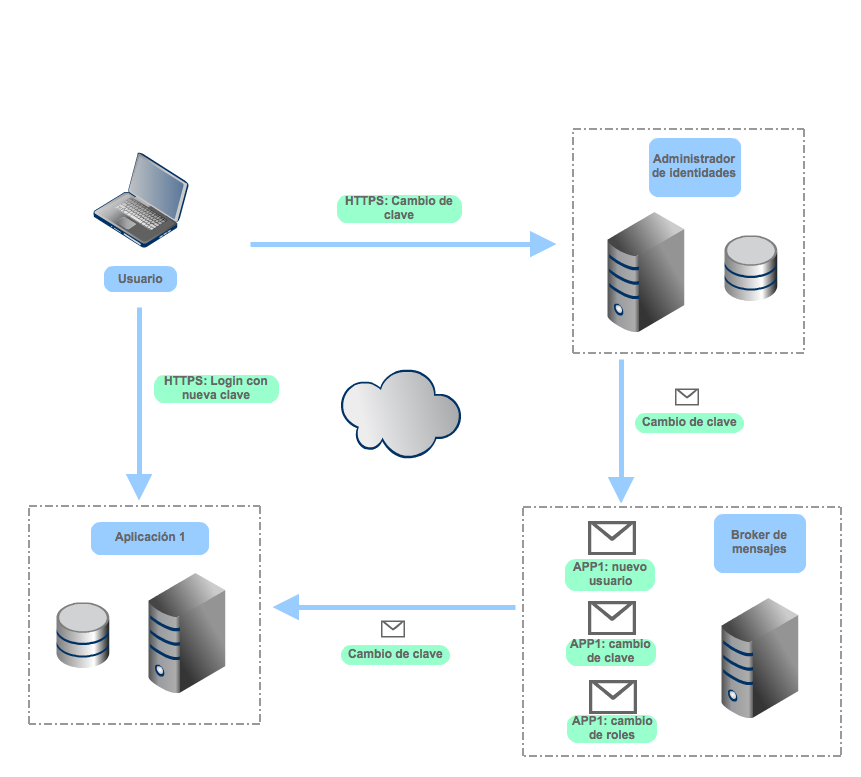
\includegraphics[scale=0.4]{./contenido/img/arquitectura.png}
\caption{Arquitectura de comunicación con el resto de las aplicaciones.}
\end{figure}

